\documentclass[tikz, border=10pt]{standalone}
\usepackage{amsmath, amssymb}
\usetikzlibrary{calc, positioning, arrows.meta, shapes.symbols, decorations.pathreplacing}

\begin{document}
	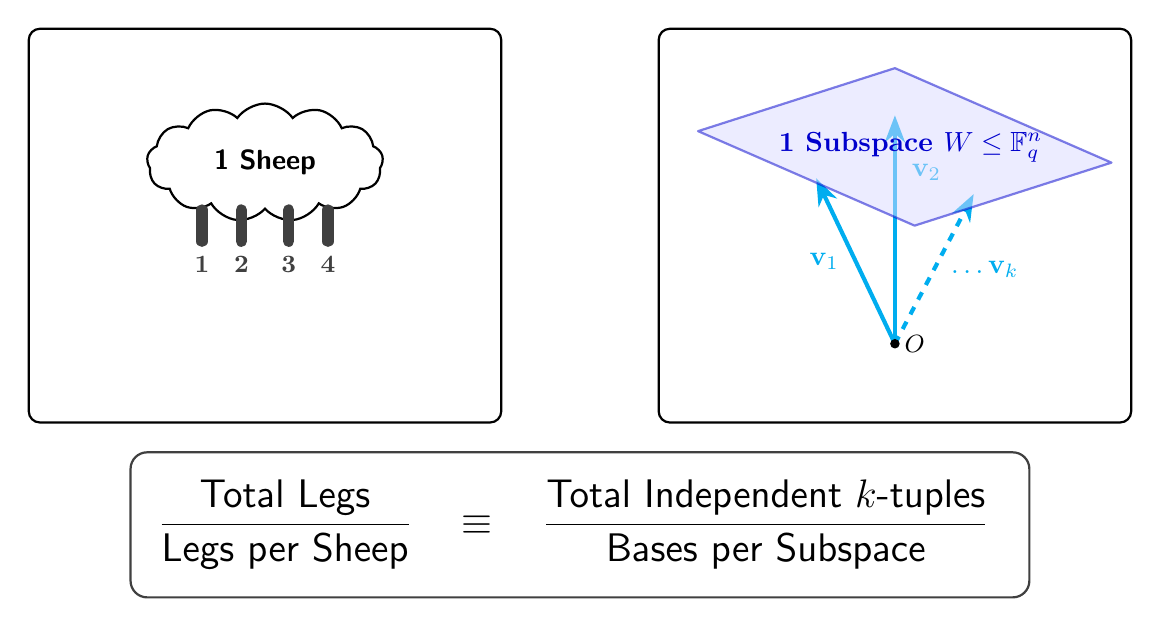
\begin{tikzpicture}[font=\sffamily]
		
		% --- LEFT PANEL: THE METAPHOR (SHEEP & LEGS) ---
		\node[draw, thick, rounded corners, minimum width=6cm, minimum height=5cm] (MetaphorBox) at (-4,0) {};
%		\node[font=\Large\bfseries, text=green!60!black] at (-4, 2.8) {The Metaphor};
		
		% Sheep Body (The 'Space')
		\node[cloud, cloud puffs=13, cloud puff arc=110, aspect=2.2, draw=black, thick, fill=white, minimum width=3cm, minimum height=1.5cm] (Sheep) at (-4, 0.8) {\textbf{1 Sheep}};
		
		% Sheep Legs (The 'Bases')
		\draw[line width=4pt, color=darkgray, line cap=round] (-4.8, 0.2) -- (-4.8, -.2) node[below, font=\small\bfseries] {1};
		\draw[line width=4pt, color=darkgray, line cap=round] (-4.3, 0.2) -- (-4.3, -.2) node[below, font=\small\bfseries] {2};
		\draw[line width=4pt, color=darkgray, line cap=round] (-3.7, 0.2) -- (-3.7, -.2) node[below, font=\small\bfseries] {3};
		\draw[line width=4pt, color=darkgray, line cap=round] (-3.2, 0.2) -- (-3.2, -.2) node[below, font=\small\bfseries] {4};
		
		% Ground line
%		\draw[thick, green!50!black] (-5.5, -1.6) -- (-2.5, -1.6);
		
%		\node[align=center, font=\small, text=darkgray] at (-4, -2.5) {
%			A single, cohesive unit\\
%			supported by a specific number\\
%			of identical structural pillars.
%		};
		
		
		% --- RIGHT PANEL: THE MATH (SUBSPACE & BASES) ---
		\node[draw, thick, rounded corners, minimum width=6cm, minimum height=5cm] (MathBox) at (4,0) {};
%		\node[font=\Large\bfseries, text=blue!60!black] at (4, 2.8) {The Mathematics};
		
		% Origin
		\coordinate (Origin) at (4, -1.5);
		
		% Basis Vectors (The 'Legs')
		\draw[->, >=Stealth, line width=1.5pt, color=cyan] (Origin) -- (3.0, 0.6) node[midway, left=2pt] {$\mathbf{v}_1$};
		\draw[->, >=Stealth, line width=1.5pt, color=cyan] (Origin) -- (4.0, 1.4) node[near end, right=2pt] {$\mathbf{v}_2$};
		\draw[->, >=Stealth, line width=1.5pt, color=cyan, dashed] (Origin) -- (5.0, 0.4) node[midway, right=2pt] {$\dots \mathbf{v}_k$};
		
		\filldraw[black] (Origin) circle (1.5pt) node[right, font=\small\bfseries] {$O$};
		
		% Subspace Platform (The 'Sheep')
		\draw[fill=blue!15, draw=blue!80!black, thick, line join=round, opacity=.5] (1.5, 1.2) -- (4, 2.0) -- (6.75, 0.8) -- (4.25, 0.0) -- cycle;
		\node[font=\bfseries, text=blue!80!black] at (4.2, 1.0) {1 Subspace $W\leq \mathbb F_q^n$};
		
%		\node[align=center, font=\small, text=darkgray] at (4, -2.5) {
%			A single $k$-dimensional space\\
%			supported (spanned) by exactly $k$\\
%			linearly independent basis vectors.
%		};
		
		
		% --- CONNECTION AND CONCLUSION ---
%		% Arrow linking the concepts
%		\draw[<->, >=Stealth, dashed, line width=2pt, color=orange!80!black] (MetaphorBox.east) -- (MathBox.west) node[midway, above, align=center, font=\bfseries, text=orange!80!black] {Conceptually\\Identical};
		
		% Bottom Summary Equation
		\node[draw=darkgray, thick, fill=white, rounded corners=6pt, minimum width=10cm, inner sep=10pt, align=center] at (0, -3.8) {
			\Large $\displaystyle \frac{\text{Total Legs}}{\text{Legs per Sheep}} \quad \equiv \quad \frac{\text{Total Independent } k\text{-tuples}}{\text{Bases per Subspace}}$
		};
		
	\end{tikzpicture}
\end{document}